\section{Otoria Hearthrust}

\begin{center}
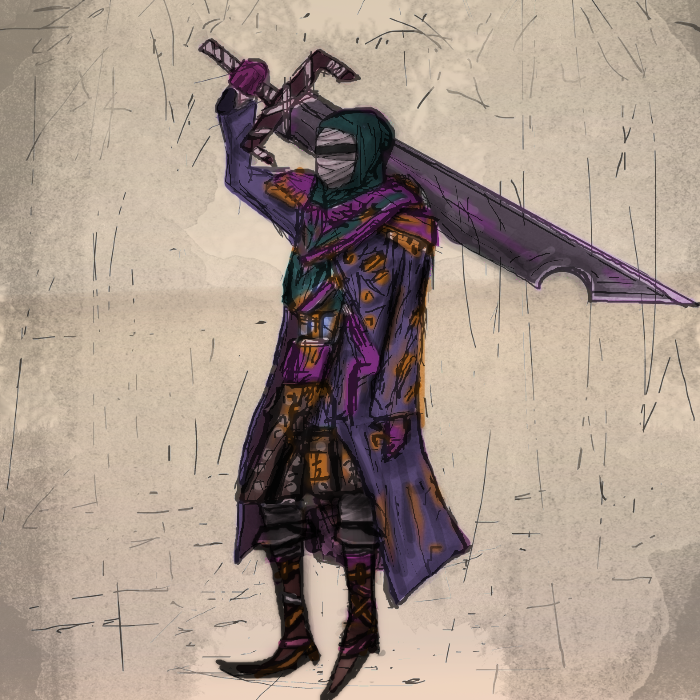
\includegraphics[width=80mm]{./content/img/otoria1.png}
\begin{figure}[h]
\end{figure}
\end{center}

\subsection*{Details}

\noindent

Race: 	Robot \\
Class: 	Fighter \\
Age: 	80 \\
Status: Deceased

\subsubsection{Background}

Lady Otoria Hearthrust arrived on the continent of Velterra from the distant land of Nanduan, where her family, the Hearthrust Dynasty, were a large, wealthy, and prominent noble house.  By Hearthrust tradition, the eldest child of each generation must be sent out into the world before coming of age, so that the family remain current, and do not stagnate, and to experience life beyond their privilege.  As a betrothed daughter, Otoria's face was covered, ``to save the world the pain of seeing, but not being able to attain, such beauty''.

She was killed in a harbour tavern in Port Averdale, choosing honour over surrender when outnumbered by scores of thugs, before being resurrected by Lazarus.

What neither Otoria nor the group initially knew was that she was not human at all, but a dwarven-crafted automaton, a robot with a soul, built with such exquisite craftsmanship that even Exme was moved to tears upon examining her inner workings.

\subsubsection{Personality and Traits}

Otoria was the group's fiercest warrior and most principled member.  She wielded a greatsword with devastating skill and fought with a code of honour that set her apart from her more morally flexible companions.  She had zero tolerance for cruelty, when Pilch murdered a surrendered Tikituk prisoner, she pinned him against the wall and delivered a chilling warning.

She was also unexpectedly nurturing, taking charge of the group's direction in early adventures and forming bonds across unlikely divides.  Her diplomatic skills were considerable, though her attempts at intimidation sometimes fell flat, she once failed to cut through a wooden pillar after delivering a dramatic speech to a crowd.

Otoria had a notable tendency to die in combat with alarming regularity, earning the epithet ``dies hard''.

\subsubsection{Relationships}

Otoria formed her closest bond with Kolo, the two sharing a heart-to-heart that transcended the usual group dynamics.  She had a complex relationship with Riphard, whose habit of ``laying hands on her for a little too long'' when healing her became a running theme.

In Nanduan, Otoria had been betrothed to an unnamed shipping magnate.  It was later revealed that she had killed the Emperor of Masuda and founded an emancipation movement for the Nanduan robot ladies, the Hearthrust Society, before fleeing to Velterra.

\subsubsection{Otoria's Story}

Otoria fought alongside the group from the Temple of Unthala through the Tower of Imota Kan, where she met her end at the blade of the lethal Lark, a singing swordswoman who beheaded her with a katana.  Her death was the group's first real loss, and it hit hard.

Exme's examination revealed Otoria's true nature as an automaton, and the group gave her a proper send-off around a campfire, keeping her mechanical remains in a special shrine.  Kolo began to tell a special story in her memory.

Otoria's legacy extended far beyond her death.  In Nanduan, the Hearthrust Society, robot ladies she had inspired and freed, continued her emancipation movement, eventually allying with the party during the Masuda campaign.  Lady Hirota Hearthrust personally rescued the group from certain death by swooping in on a mechanical eagle, and the Society's female ninja riders on mechanical eagles joined the final assault on Seven's Spire, fighting alongside the alliance army to break the Church's power.

\vspace{5mm}

\textit{In loving memory of Lady Otoria Hearthrust. 2017--2017.}


\begin{center}
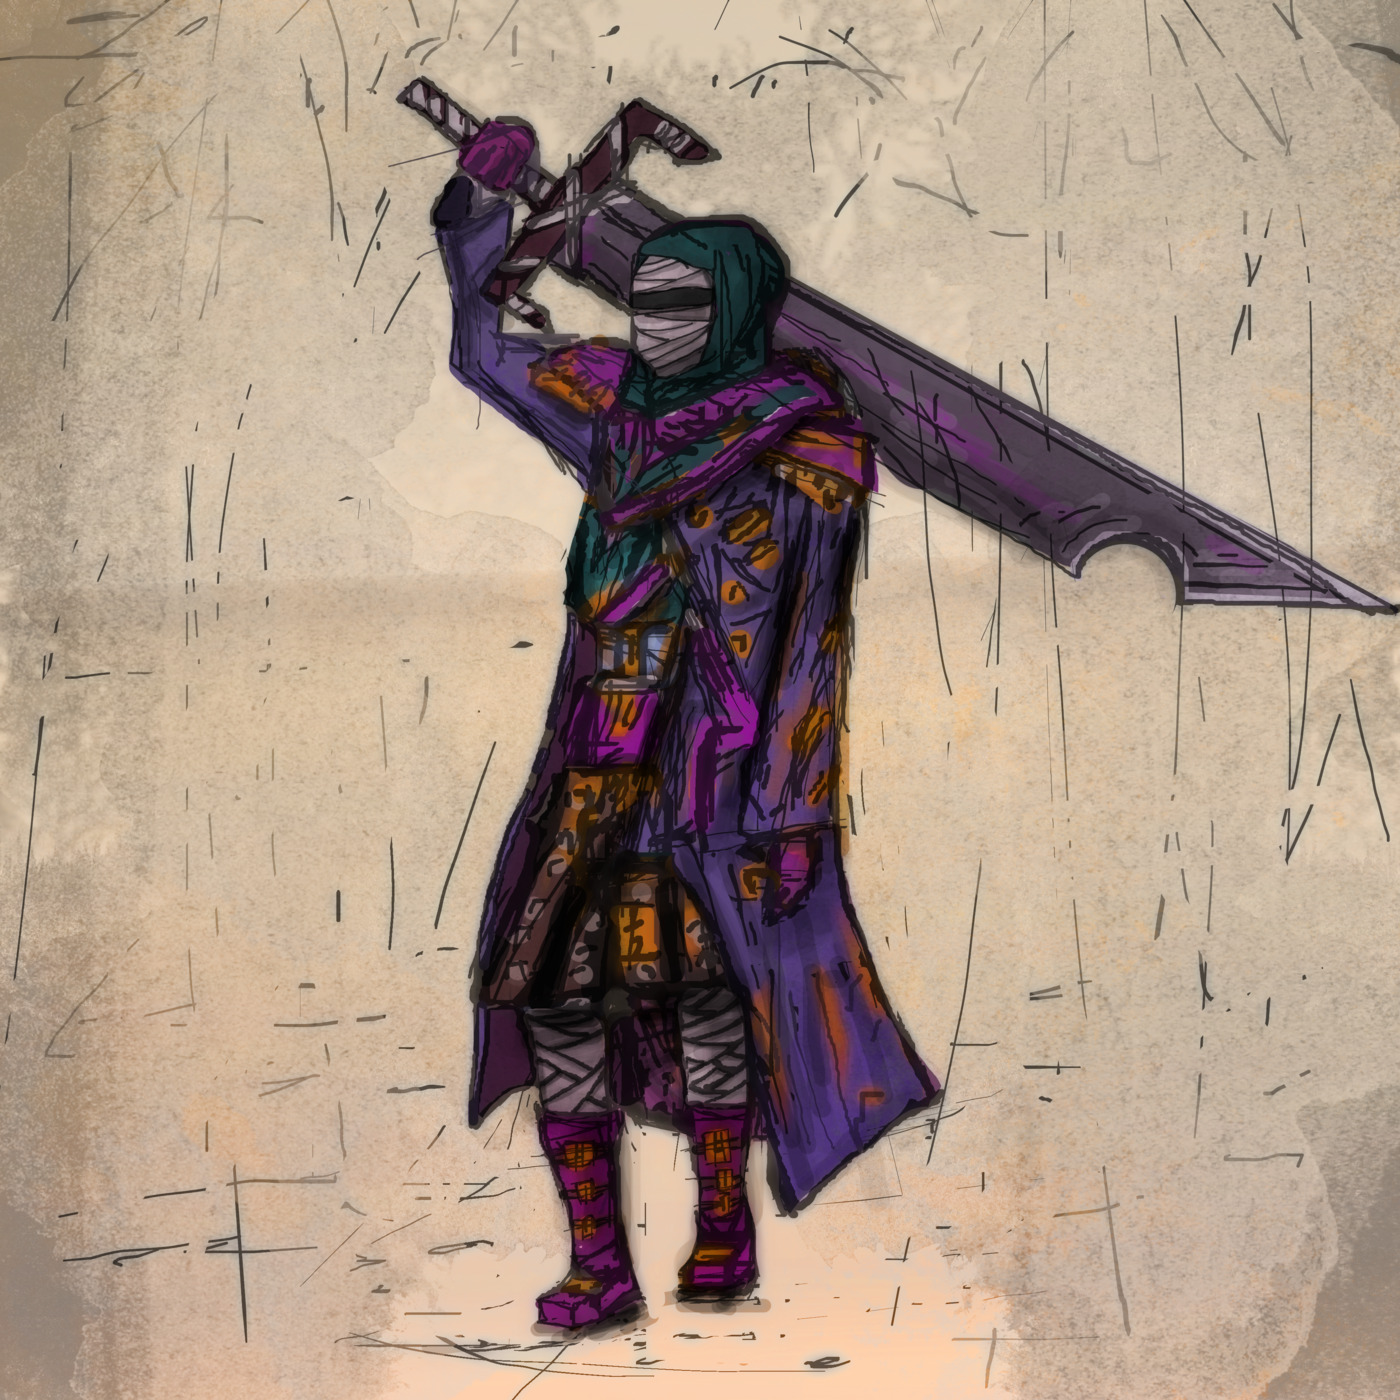
\includegraphics[width=80mm]{./content/img/reddit/otoriaOriginal.jpg}\\
\textit{Lady Otoria's original character art, February 2017}
\end{center}

\clearpage
